\section{Unsuccessful Trials}
We started with and settled on using \texttt{LBPH} for feature extraction and \texttt{SVM} for classfication.
They both gave around 80\% accuracy at the beginning, and with tuning for preprocessing the accuracy reached \~99\% over large tests.
During that, part of the team were testing other feature extraction methods and classfiers.

We tried to extract \emph{Histogram of Oriented Gradients} (\texttt{HOG}) features.
Using \texttt{HOG} gave very low accuracy (\~46\%) on 15 test cases.
We extracted \texttt{HOG} from the binary image and then gray image, with no visible changes.

Then we tried to extract the \emph{Hu Moments} that are used to describe the shapes.
We extracted \emph{Hu Moments} from each binary line in the image.
Using \emph{Hu Moments} with \texttt{SVM} gave accuracies lower than that of \texttt{HOG} on the same number of test cases.

Being very low made sense, because we tried to describe the shape of the whole line.
So we tried to extract \emph{Hu Moments} from a sliding window of size $13\times13$.
This gave accuracy of \~48\% on 15 tests.
On some lucky iterations, it gave \~80\%.

Then we tried to mix both \texttt{HOG} features and \emph{Hu Moments}.
This gave us accuracy of \~66\% on 15 tests.
It wasn't slower than only \texttt{HOG}, because we used subset of both features.

By this time, \texttt{LBPH} reached \~99\% accuracy on 200 tests.
So we abandoned optimizing the feature extraction anymore.

Figure \ref{fig:unsuccBar} shows the accuracies for the different features.

\begin{figure}
    \centering
    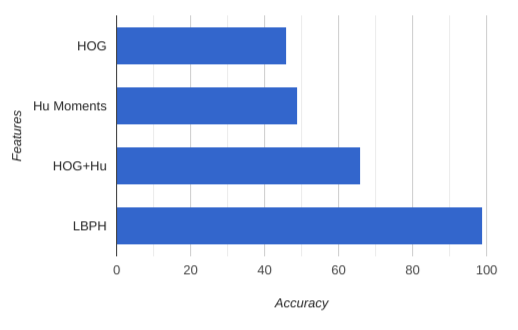
\includegraphics[width=0.9\linewidth]{figures/unsuccBar.png}
    \caption{Feature Extraction Methods Accuracy for 15 tests.}
    \label{fig:unsuccBar}
\end{figure}

We tried another classfication method beside \texttt{SVM}.
We used \emph{K-Nearest Neighbours} (\texttt{KNN}), and it gave the same accuracies of \texttt{LBPH} but was noticably slower.
It made sense that \texttt{KNN} is slower, because it iterates over the features multiple times to find the mean and cluster them.
